%%%%%%%%%%%%%%%%%%%%%%%%%%%%%%%%%%%%%%%%%
% Beamer Presentation
% Titto Thomas
%%%%%%%%%%%%%%%%%%%%%%%%%%%%%%%%%%%%%%%%%

\documentclass{beamer}

\mode<presentation> {

\usetheme{Antibes}
\usecolortheme{beaver}
\setbeamertemplate{footline}[page number] % To replace the footer line in all slides with a simple slide count uncomment this line
\setbeamertemplate{navigation symbols}{}
}

\usepackage{graphicx} % Allows including images
\usepackage{booktabs} % Allows the use of \toprule, \midrule and \bottomrule in tables
\usepackage{minted}
\usepackage[titletoc]{appendix}
%----------------------------------------------------------------------------------------
%	TITLE PAGE
%----------------------------------------------------------------------------------------

\title[Scan chain for DE0-Nano systems]{Scan chain based test setup \\ for DE0-Nano based systems} % The short title appears at the bottom of every slide, the full title is only on the title page

\author{Titto Thomas} % Your name
\institute[EE 705] % Your institution as it will appear on the bottom of every slide, may be shorthand to save space
{
Wadhwani Electronics Laboratory \\ EE Dept. IIT Bombay \\ % Your institution for the title page
\medskip
\textit{tittothomas@iitb.ac.in} % Your email address
}
\date{\today} % Date, can be changed to a custom date

\begin{document}

\begin{frame}
\titlepage % Print the title page as the first slide
\end{frame}

%----------------------------------------------------------------------------------------
%	PRESENTATION SLIDES
%----------------------------------------------------------------------------------------

%------------------------------------------------
\section{Introduction} % Introduction Section
\subsection{Scan Chain}
\begin{frame}
\frametitle{Scan Chain}

\begin{figure}[h!]
\centering
% XCircuit output "scanChain.tex" for LaTeX input from scanChain.ps
\def\putbox#1#2#3#4{\makebox[0in][l]{\makebox[#1][l]{}\raisebox{\baselineskip}[0in][0in]{\raisebox{#2}[0in][0in]{\scalebox{#3}{#4}}}}}
\def\rightbox#1{\makebox[0in][r]{#1}}
\def\centbox#1{\makebox[0in]{#1}}
\def\topbox#1{\raisebox{-0.60\baselineskip}[0in][0in]{#1}}
\def\midbox#1{\raisebox{-0.20\baselineskip}[0in][0in]{#1}}
   \scalebox{0.5}{
   \normalsize
   \parbox{6.16667in}{
   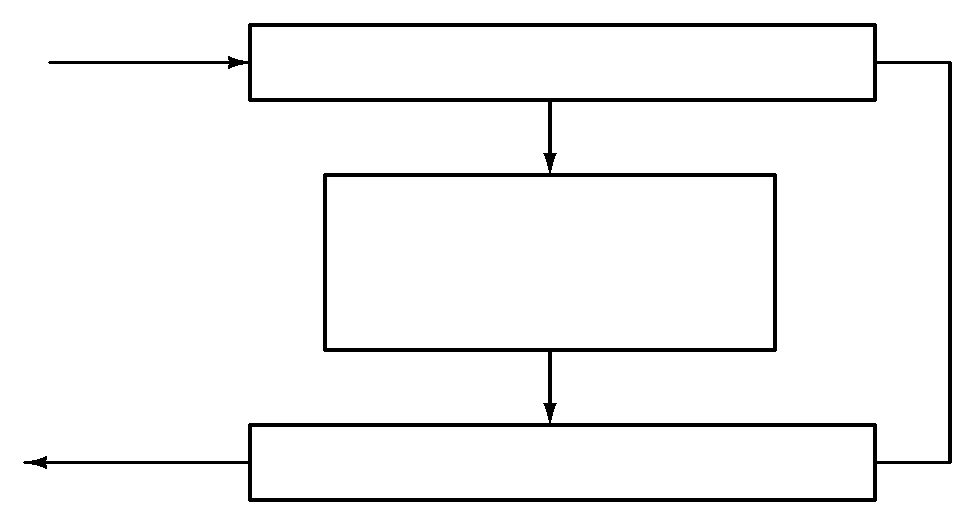
\includegraphics[scale=1]{scanChain.eps}\\
   % translate x=704 y=320 scale 0.38
   \putbox{3.31in}{1.64in}{1.20}{DUT}%
   \putbox{0.22in}{3.06in}{1.20}{data in}%
   \putbox{0.22in}{0.47in}{1.20}{data out}%
   \putbox{3.64in}{2.47in}{1.20}{input}%
   \putbox{3.64in}{0.81in}{1.20}{output}%
   } % close 'parbox'
   } % close 'scalebox'
   \vspace{-\baselineskip} % this is not necessary, but looks better

\end{figure}

\begin{itemize}
\item Scan chain is a technique used for testing the hardware systems.
\item a simple way to set the inputs for the system and observe their outputs.
\item It consists of two shift registers and their control signals.
\end{itemize}
\end{frame}
%------------------------------------------------
% A subsection can be created just before a set of slides with a common theme to further break down your presentation into chunks
\subsection{JTAG}

\begin{frame}
\frametitle{Joint Test Action Group (JTAG)}

\begin{figure}[h!]
\centering
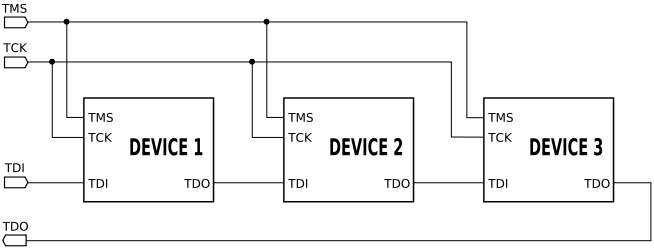
\includegraphics[scale=0.3]{jtagWiki.png}
\end{figure}

\begin{itemize}
\item Started as a method to test PCB boards, currently used as an industry standard for testing.
\item It has a boundary scan architecture, i.e all the input and output pins are linked together in a set called the Boundary Scan chain.
\item A simplified version of standard JTAG is proposed here for testing designs on the DE0-Nano board.
\end{itemize}

\begin{flushright}
\begin{scriptsize}
\textit{www.wikipedia.org/wiki/Joint\_Test\_Action\_Group}
\end{scriptsize}
\end{flushright}

\end{frame}

%------------------------------------------------
\section{Test Setup}
\subsection{Test Setup}

\begin{frame}
\frametitle{Main blocks}

\begin{itemize}
\item Has three main parts.

\begin{itemize}
\item \texttt{Python Script} : Gets the command inputs from the user in a text file.
\item \texttt{Microcontroller(ATxMega128)} : Convert these commands into a set of signals for the DE0-Nano board.
\item \texttt{DE0-Nano board} : Contains both the DUT and the proposed scan chain.
\end{itemize}

\item The PC communicates to the microcontroller through a USB link , with a predefined standard data transfer scheme.
\item The microcontroller will translate the commands, and generate corresponding signals through it's port pins.
\end{itemize}

\end{frame}

\begin{frame}
\frametitle{Block Diagram}

\begin{figure}[h!]
\centering
% XCircuit output "scan_main.tex" for LaTeX input from scan_main.ps
\def\putbox#1#2#3#4{\makebox[0in][l]{\makebox[#1][l]{}\raisebox{\baselineskip}[0in][0in]{\raisebox{#2}[0in][0in]{\scalebox{#3}{#4}}}}}
\def\rightbox#1{\makebox[0in][r]{#1}}
\def\centbox#1{\makebox[0in]{#1}}
\def\topbox#1{\raisebox{-0.60\baselineskip}[0in][0in]{#1}}
\def\midbox#1{\raisebox{-0.20\baselineskip}[0in][0in]{#1}}
   \scalebox{1}{
   \normalsize
   \parbox{6.75in}{
   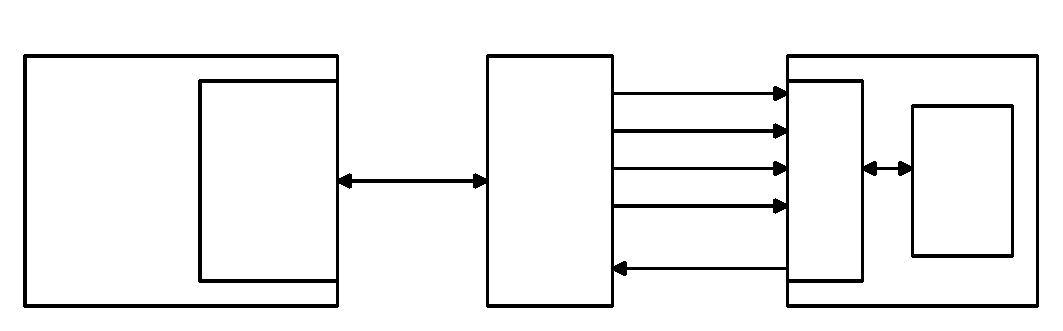
\includegraphics[scale=0.9]{scan_main.eps}\\
   % translate x=1040 y=64 scale 0.38
   \putbox{0.78in}{1.65in}{1.20}{PC}%
   \putbox{2.7in}{1.65in}{1.20}{ATxMega128}%
   \putbox{4.8in}{1.65in}{1.20}{DE0-Nano}%
   \putbox{1.23in}{0.9in}{1.20}{Python}%
   \putbox{1.28in}{0.7in}{1.20}{Script}%
   \putbox{2.02in}{0.6in}{1.20}{USB link}%
   \putbox{3.9in}{1.38in}{1.20}{{\small TDI}}%
   \putbox{3.87in}{1.15in}{1.20}{{\small TCLK}}%
   \putbox{3.9in}{0.92in}{1.20}{{\small TMS}}%
   \putbox{3.87in}{0.68in}{1.20}{{\small TRST}}%
   \putbox{3.9in}{0.11in}{1.20}{{\small TDO}}%
   \putbox{4.8in}{0.35in}{1.20}{\rotatebox{-270}{Scan Chain}}%
   \putbox{5.48in}{0.81in}{1.20}{DUT}%
   } % close 'parbox'
   } % close 'scalebox'
   \vspace{-\baselineskip} % this is not necessary, but looks better

\end{figure}

\end{frame}

\begin{frame}
\frametitle{Interface Signals}

\begin{itemize}
\item The tester hardware contains the scan chain and the controller ( TAP controller ) that provides necessary control signals to it.
\item The interface signals of this top level system would be

\begin{itemize}
\item \texttt{TDI} : The serial test data input to be loaded in the scan chain.
\item \texttt{TMS} : The commands for the TAP ( Test Access Port ) controller are passed serially through this pin.
\item \texttt{TCLK} : The clock reference forin design for testing all the other communication lines.
\item \texttt{TRST} : Pin to reset the TAP controller at any instant.
\item \texttt{TDO} : The serial data output from the scan chain.
\end{itemize}

\end{itemize}

\end{frame}

%----------------------Adding scan chain to design-----------------------------------------

\section{Adding scan chain to your exisitng VHDL design}
\subsection{Adding scan chain}
\begin{frame}
\frametitle{Adding scan chain}

\begin{figure}[h!]
\centering
% XCircuit output "DUT.tex" for LaTeX input from DUT.ps
\def\putbox#1#2#3#4{\makebox[0in][l]{\makebox[#1][l]{}\raisebox{\baselineskip}[0in][0in]{\raisebox{#2}[0in][0in]{\scalebox{#3}{#4}}}}}
\def\rightbox#1{\makebox[0in][r]{#1}}
\def\centbox#1{\makebox[0in]{#1}}
\def\topbox#1{\raisebox{-0.60\baselineskip}[0in][0in]{#1}}
\def\midbox#1{\raisebox{-0.20\baselineskip}[0in][0in]{#1}}
   \scalebox{1}{
   \normalsize
   \parbox{6.66667in}{
   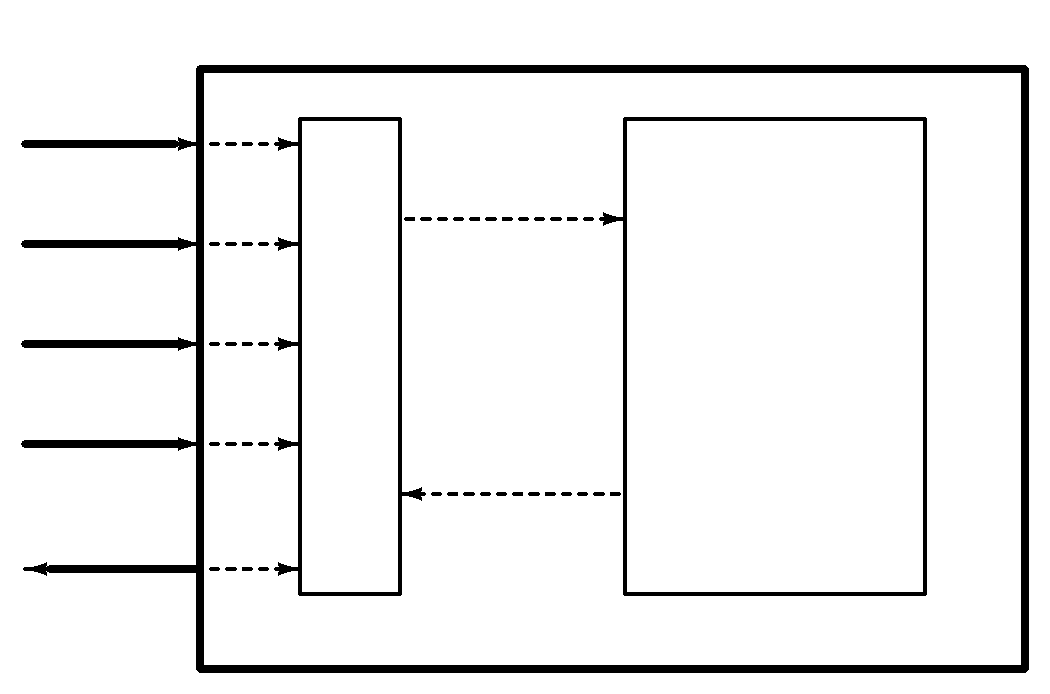
\includegraphics[scale=0.75]{DUT.eps}\\
   % translate x=1024 y=352 scale 0.38
   \putbox{3.59in}{1.56in}{1.20}{DUT}%
   \putbox{2.19in}{2.46in}{1.20}{dut\_in}%
   \putbox{2.19in}{0.66in}{1.20}{dut\_out}%
   \putbox{0.35in}{2.72in}{1.20}{TDI}%
   \putbox{0.27in}{2.22in}{1.20}{TCLK}%
   \putbox{0.31in}{1.73in}{1.20}{TMS}%
   \putbox{0.22in}{1.22in}{1.20}{TRST}%
   \putbox{0.31in}{0.6in}{1.20}{TDO}%
   \putbox{1.58in}{1.16in}{1.20}{\rotatebox{-270}{Scan Chain}}%
   \putbox{3.94in}{3.12in}{1.20}{mySystem}%
   } % close 'parbox'
   } % close 'scalebox'
   \vspace{-\baselineskip} % this is not necessary, but looks better

\end{figure}

\end{frame}

\begin{frame}
\frametitle{Adding scan chain (Contd.)}
\begin{itemize}
\item DUT should first be tested in gate level simulation and verified to be working.
\item user has to write a top level entity (shown as \texttt{mySystem}) which contains the DUT and \texttt{Scan\_Chain} module as component.
\item \texttt{mySystem} should have 5 interface signals, \texttt{TDI}, \texttt{TMS}, \texttt{TCLK}, \texttt{TRST} and \texttt{TDO}.
\end{itemize}
\end{frame}

\subsection{Scan Chain specifications}

\begin{frame}[fragile]
\frametitle{Scan Chain specifications}

\begin{minted}[fontsize=\footnotesize]{vhdl}
entity Scan_Chain is
  generic (
    in_pins : integer; -- Number of input pins
    out_pins : integer -- Number of output pins
  );
  port (
    TDI : in std_logic;  -- Test Data In
    TDO : out std_logic;  -- Test Data Out
    TMS : in std_logic;  -- TAP controller signal
    TCLK : in std_logic;  -- Test clock
    TRST : in std_logic;  -- Test reset
    dut_in : out std_logic_vector(in_pins-1 downto 0);  
    						-- Input for the DUT
    dut_out : in std_logic_vector(out_pins-1 downto 0);  
    						-- Output from the DUT
  );
end Scan_Chain;
\end{minted}

\end{frame}

\begin{frame}
\frametitle{Scan Chain specifications (Contd.)}

\begin{itemize}
\item Scan chain has two configurable parameters ( \texttt{in\_pins} and \texttt{out\_pins} ) indicating the number of input and output bits to the DUT, which can be generic mapped.
\item It also has one output (\texttt{dut\_in}) and one input (\texttt{dut\_out}) that should be connected to the DUT.
\item Internally it contains an FSM ( that implements the TAP Controller ), one input scan register and one output scan register.
\end{itemize}

\end{frame}

\subsection{Reference Implementation}

\begin{frame}
\frametitle{Reference Implementation : Counter}
\begin{columns}[l] % The "c" option specifies centered vertical alignment while the "t" option is used for top vertical alignment

\column{.5\textwidth} % Left column and width
\begin{figure}[h!]
\centering
% XCircuit output "Counter.tex" for LaTeX input from Counter.ps
\def\putbox#1#2#3#4{\makebox[0in][l]{\makebox[#1][l]{}\raisebox{\baselineskip}[0in][0in]{\raisebox{#2}[0in][0in]{\scalebox{#3}{#4}}}}}
\def\rightbox#1{\makebox[0in][r]{#1}}
\def\centbox#1{\makebox[0in]{#1}}
\def\topbox#1{\raisebox{-0.60\baselineskip}[0in][0in]{#1}}
\def\midbox#1{\raisebox{-0.20\baselineskip}[0in][0in]{#1}}
   \scalebox{1}{
   \normalsize
   \parbox{5.16667in}{
   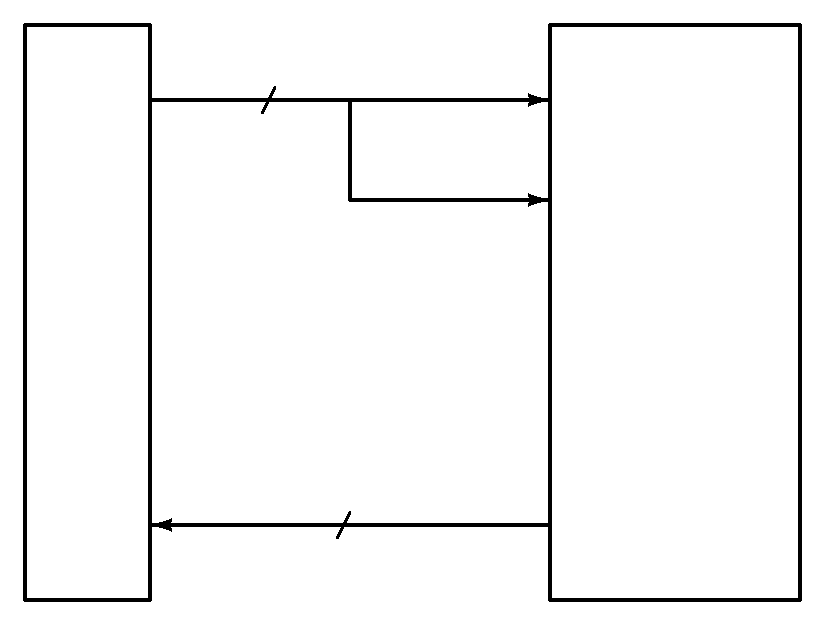
\includegraphics[scale=0.8]{Counter.eps}\\
   % translate x=672 y=512 scale 0.38
   \putbox{0.78in}{2.86in}{1.20}{\texttt{dut\_in[1:0]}}%
   \putbox{1.97in}{2.86in}{1.20}{\texttt{dut\_in[1]}}%
   \putbox{1.97in}{2.32in}{1.20}{\texttt{dut\_in[0]}}%
   \putbox{1.36in}{0.62in}{1.20}{\texttt{dut\_out[7:0]}}%
   \putbox{2.94in}{0.4in}{1.20}{\texttt{count}}%
   \putbox{2.94in}{2.65in}{1.20}{\texttt{reset}}%
   \putbox{2.94in}{2.1in}{1.20}{\texttt{clock}}%
   \putbox{0.35in}{1.16in}{1.20}{\rotatebox{-270}{Scan Chain}}%
   \putbox{3.2in}{1.4in}{1.20}{Counter}%
   } % close 'parbox'
   } % close 'scalebox'
   \vspace{-\baselineskip} % this is not necessary, but looks better

\end{figure}

\column{.6\textwidth} % Right column and width
\begin{itemize}
\item The counter has two single bit inputs ( \texttt{clock} and \texttt{reset} ) and an 8 bit single output ( \texttt{count}).
\item Here, the \texttt{dut\_in} will be 2 bits ( one for each of the inputs ) and \texttt{dut\_in} will be same as \texttt{count}.
\item The top level VHDL description of this system is given in supporting document.
\end{itemize}

\end{columns}
\end{frame}

%------------------------------------------------
\section{Hardware Interfacing}
%------------------------------------------------
\begin{frame}
\frametitle{Hardware connections}

\begin{itemize}
\item Next step is to make physical connections between the host PC, microcontroller board and the user module (on DE0-Nano).
\item The microcontroller board is PtX-128 ( ATxMega128 based ) developed in WEL lab, IITB. Connect it to the PC.
\item The following connections between the microcontroller board and the DE0-Nano need to be made

\begin{itemize}
\item \texttt{TRST} (DE0-Nano) to PD4 (PORTD.4)
\item \texttt{TDI} (DE0-Nano) to PD0 (PORTD.0)
\item \texttt{TMS} (DE0-Nano) to PD1 (PORTD.1)
\item \texttt{TCLK} (DE0-Nano) to PD5 (PORTD.5)
\item \texttt{TDO} (DE0-Nano) to PC0 (PORTC.0)
\end{itemize}

\end{itemize}
\end{frame}
%------------------------------------------------
\section{Input file format}
%------------------------------------------------
\subsection{Input file format}
\begin{frame}
\frametitle{Input file format}

\begin{itemize}
\item For testing the hardware, the user has to provide input combinations, their expected results and the time duration of execution.
\item They should be written as commands in a text file and passed to the python script for test execution.
\item These commands are derived from the Serial Vector Format (SVF), usually used in JTAG boundary scan.
\item Only two commands are required for the current implementation.

\end{itemize}
\end{frame}

\subsection{Input commands}
\begin{frame}
\frametitle{SDR}
\texttt{SDR $<in\:pins>$ TDI($<input>$) $<out\:pins>$ TDO($<output>$) MASK($<mask\:bits>$)}
\vspace*{0.3cm}
\begin{itemize}
\item This Serial Data Register instruction is for carrying out a data scan in process.
\item $in\:pins$ \& $out\:pins$ contains the number of input and output bits respectively.
\item $input$ \& $output$ contains the input combination to be applied and it's expected output combination respectively.
\item  $mask\:bits$ are used to specify if any of the output bits are not important and could be taken as don't care
\end{itemize}
Example : \texttt{SDR 2 TDI(0) 8 TDO(00) MASK(FF)}\\
\textit{Note} : If the scanned output should not be compared, then all the $mask\:bits$ should be kept as 0.
\end{frame}

\begin{frame}
\frametitle{RUNTEST}
\texttt{RUNTEST $<delay>$ SEC}
\begin{itemize}
\item As the previous instruction loads the input and samples the output, this instruction is used to apply the input combination to the DUT and wait for $delay$ seconds.
\end{itemize}
Example : \texttt{RUNTEST 60 SEC}
\begin{itemize}
\item The $input$, $output$ and $mask\:bits$ are to be written as hexadecimel numbers ( uppercase for alphabets ).
\item An example input file is given in the supporting document.
\end{itemize}

\end{frame}
%------------------------------------------------
\section{Running the Python script}
%------------------------------------------------

\begin{frame}
\frametitle{Running the Python script}
\begin{itemize}
\item First install pyUSB library on the PC by the following steps.

\begin{itemize}
\item Download pyUSB v1.0 from the site ``\textit{http://sourceforge.net/projects/pyusb/}"
\item Follow the steps in the README document to install libusb and pyusb v1.0 on linux.
\end{itemize}

\item Now run the \texttt{scan.py} script with the following command.
\vspace*{0.5cm}
\begin{center}
\texttt{\$ sudo scan.py \textit{<input file>} \textit{<output file>}} 
\end{center}
\vspace*{0.5cm}
Where \textit{input file} contains all the commands to be executed, and \textit{output file} should be an empty file for storing the results.
\end{itemize}

\end{frame}

%------------------------------------------------
\section{The End}
\begin{frame}
\Huge{\centerline{Thank You}}
\end{frame}

%----------------------------------------------------------------------------------------

\end{document}